\documentclass{article}
\usepackage{../fasy-hw}
\usepackage{graphicx}

%% UPDATE these variables:
\renewcommand{\hwnum}{3}
\title{Discrete Structures, Homework \hwnum}
\author{Peyton Meeks (Peyton Meeks)}
\collab{n/a}
\date{due: 19 February 2021}

\begin{document}

\maketitle

This homework assignment should be
submitted as a single PDF file both to D2L and to Gradescope.

General homework expectations:
\begin{itemize}
    \item Homework should be typeset using LaTex.
    \item Answers should be in complete sentences and proofread.
    \item You will not plagiarize.  \item List collaborators at the start of each question using the \texttt{collab} command.
    \item Put your answers where the \texttt{todo} command currently is (and
        remove the \texttt{todo}, but not the word \texttt{Answer}).
\end{itemize}

% ============================================
% ============================================
\collab{n/a} \nextprob{Negations}
% ============================================
% ============================================
Negate the following statements:

\begin{enumerate}

    \item Each ``Clean 'Cat Kit''  contains a cloth mask and a refillable hand
        sanitizer.

        \paragraph{Answer}
        There exists a ``Clean 'Cat Kit" that does not contain a cloth mask or a refillable hand sanitizer.

    \item There exists a boat docked in New Jersey that I have steered.

        \paragraph{Answer}
        For every boat docked in New Jersey there is one I have not steered.

    \item There exists an island in the Ohio River with a bowling alley and a
        university track field.

        \paragraph{Answer}
        For every island in the Ohio River there is one that does not have a bowling alley or a university track field.

    \item Both my sister and I can climb every route at Spire.

        \paragraph{Answer}
        There exists a route at the Spire which neither my sister or I can climb.

\end{enumerate}

% ============================================
% ============================================
\collab{Shreya Deb} \nextprob{Definitions}
% ============================================
% ============================================
Use the definitions provided in the course textbook to prove that every prime
number except~$2$ is odd.

\paragraph{Answer}

By the definition of prime numbers: for some interger $n$, if $n>1$ and for all other positve intergers $(r,s) n=rs$ then $r$ or $s$ equals $n$ and $1$. Say there exists a prime integer $q>2$, then by the definition of an even number ``for all intergers $n$ and $k$, $n$ is even if $n=2k$.", $q$ is even if $q/k=2$. Since $q$ is prime this is not possible, therefore no even number other than $2$ exists.
%
% ============================================
% ============================================
\collab{\todo{}}
\nextprob{Four Colors Suffice}
% ============================================
% ============================================
Read Chapters $2$ and $3$ of \emph{Four Colors Suffice} and answer the following questions:

\begin{enumerate}

    \item Who are the Austrian(s) mentioned in Chapters $1$--$3$, and what was their
        contribution mentioned in the book?

        \paragraph{Answer}
       Heinrich Tietze, provided an example that if maps are in the 3rd dimension then they require as many colors as there are countries.

    \item Write a statement of the four color theorem using a universal
        quantifier.

        \paragraph{Answer}
        For all maps $m$ with $f$ number of faces, the number of colors $c$ required to cover each face so that no touching face has the same color is $c \leq 4$.

    \item What is the definition of a $k$-coloring of a graph?

        \paragraph{Answer}
        A $k$ coloring of a graph is a graph where the vertices are colored in a way that no adjacent vertices have the same color.

    \item Prove or disprove: all plane graphs are three-colorable.

        \paragraph{Answer}
		Say there exists a plane graph that is not three colorable. By the Four Color Therom we know that at most 4 colors are needed to color a plane graph. That means that not all graphs will require 4 colors but not all will be satisfied with only three either.        

    \item Assuming the four color theorem holds, prove or disprove: six colors
        suffice to color a plane graph.

        \paragraph{Answer}
        Since four colors suffice for all plane graphs then six colors would more than suffice to the point of redundancy.

    \item Give an example of a map with at least five faces that has a
        two-coloring.  Be sure to provide a coloring as evidence that the map is
        two-colorable.

        \paragraph{Answer}
        \begin{figure}[h]
			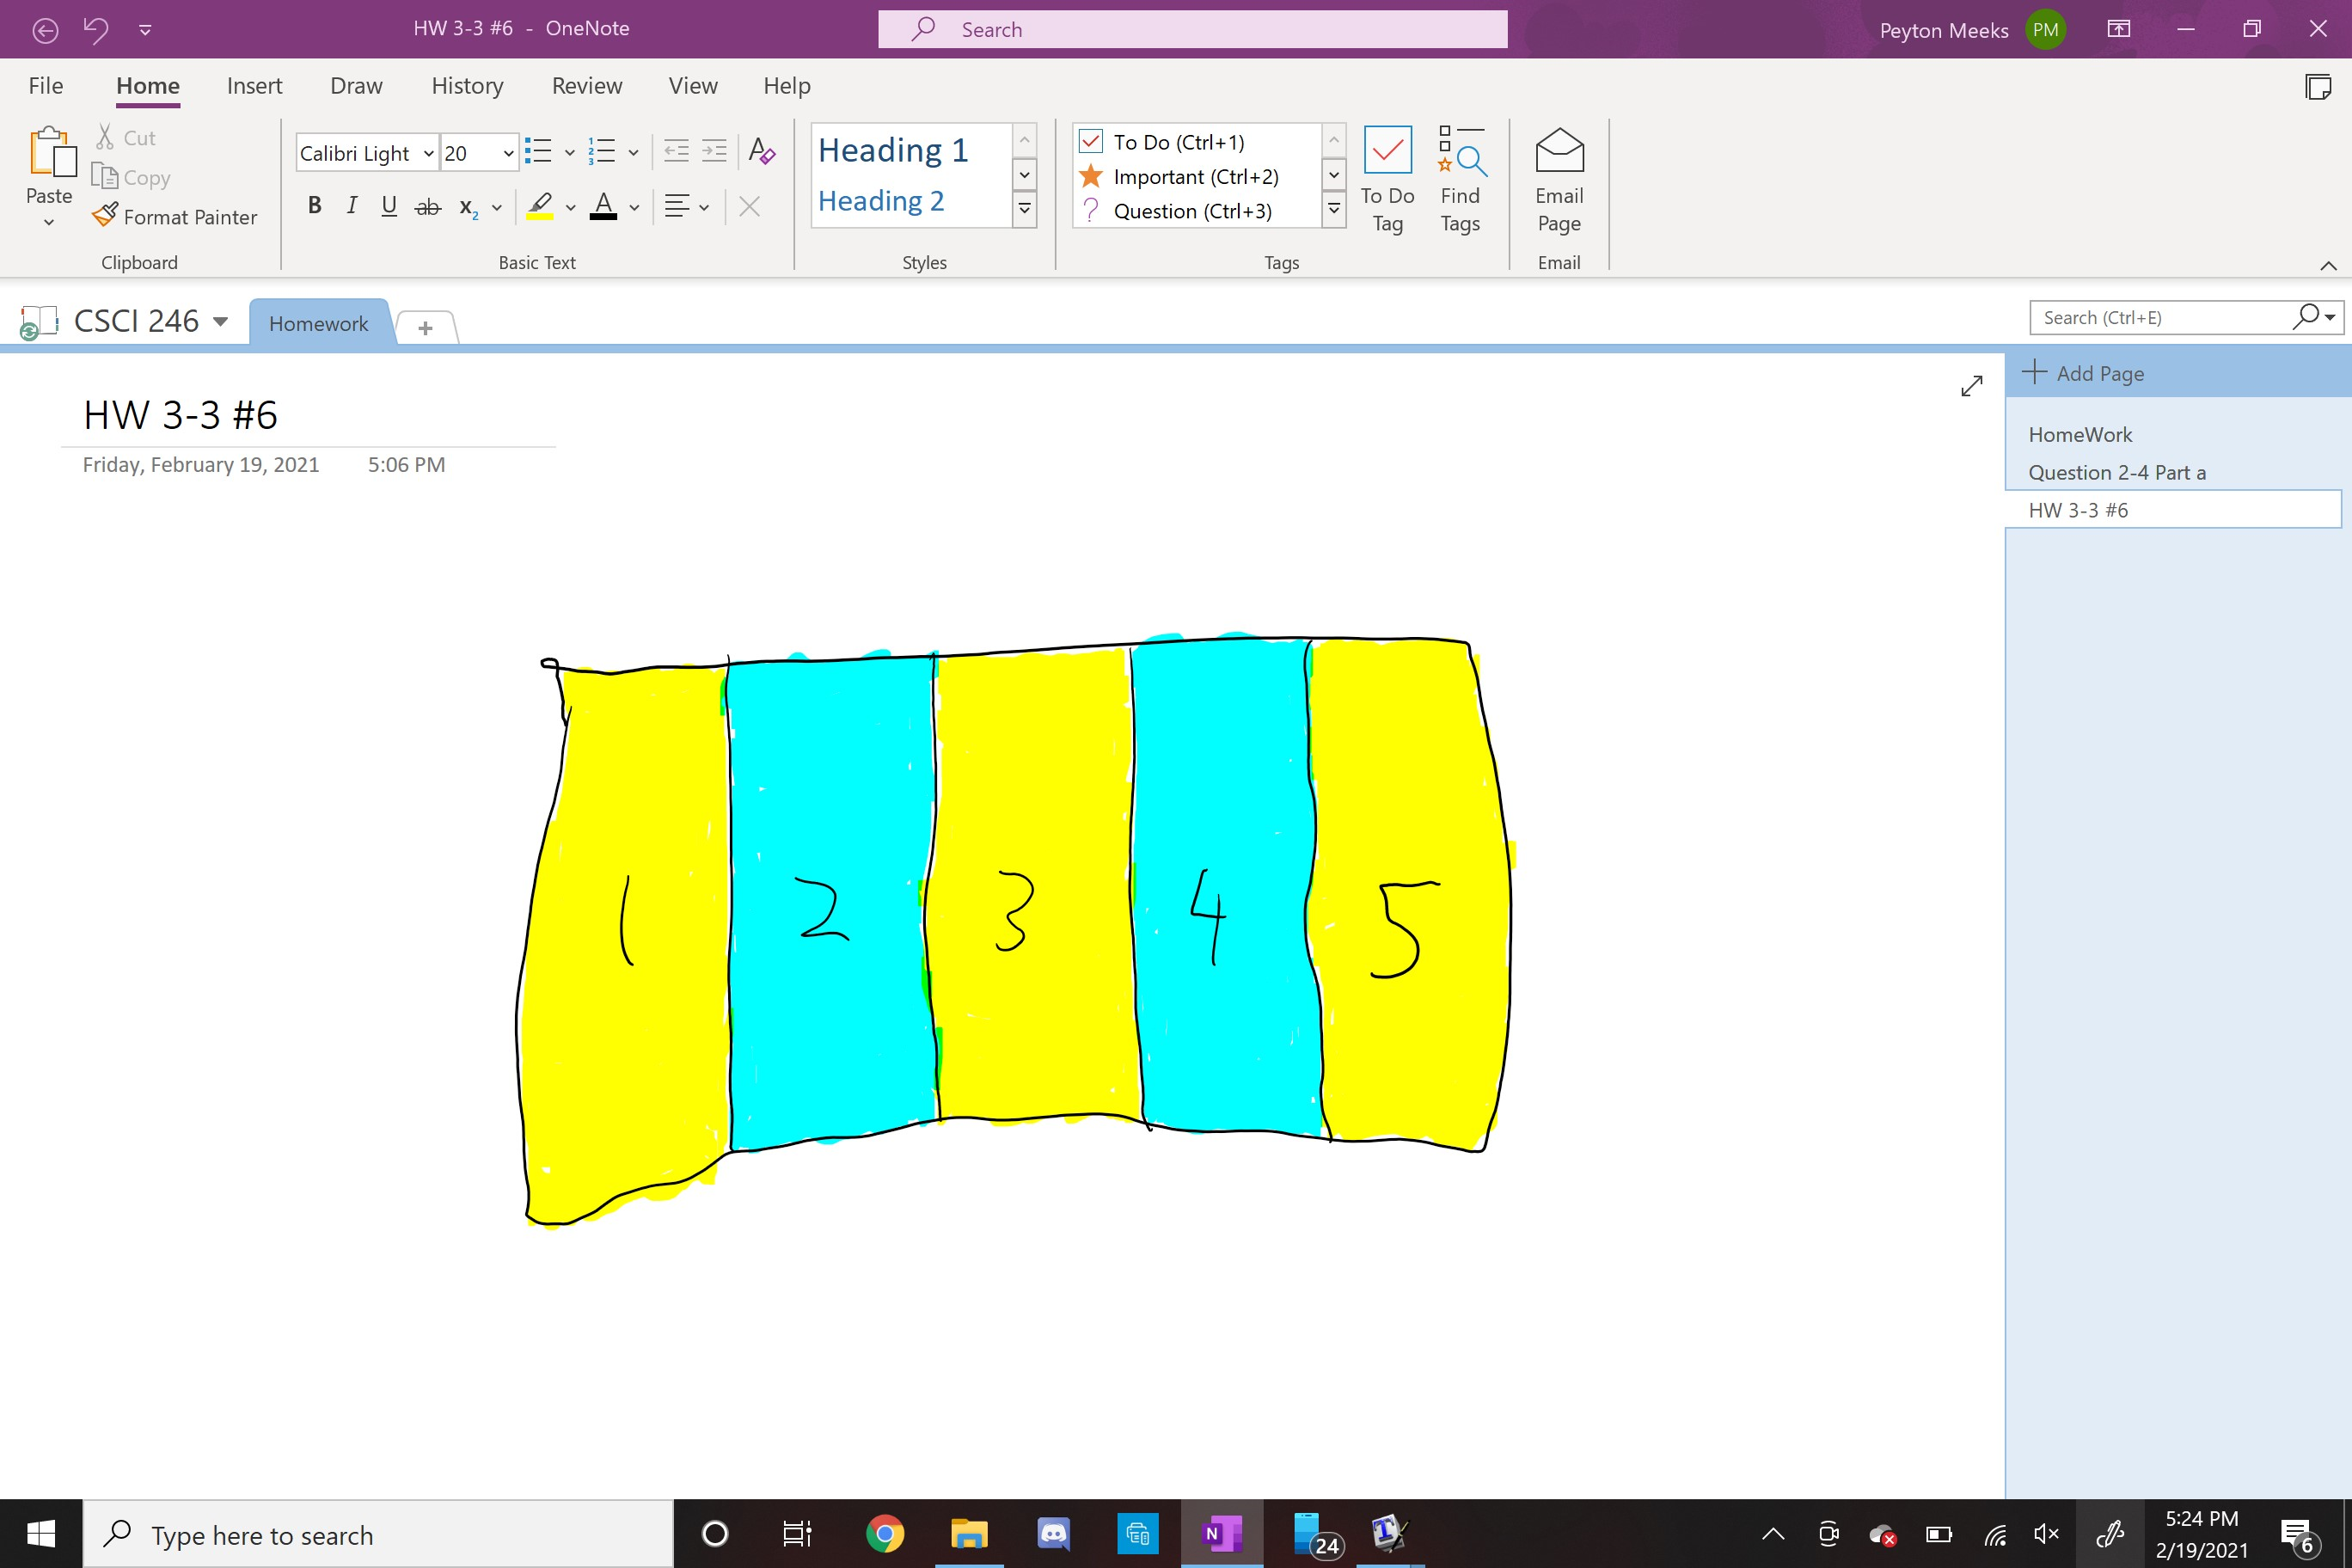
\includegraphics[width=0.5\textwidth]{HW 3-3_6}
		\end{figure}

    \item Euler's formula states that if we have a map on the sphere or plane
        and count the exterior face as a face, then F-E+V=2.  Does this equation
        hold if the map is drawn on a M\"obius band? Why or why not? (Note:
        here, the boundary of the M\"obius band must be represented in the graph
        defining the map, and no ``country'' can be on the same side of a single
        edge.)

        \paragraph{Answer}
       No it does not, becuase when you create the M\"obius band Euler's Formula is $2-1+0$, which does not equal $2$ since the band only has one face and one edge within it and no verticies.

    \item In your own words, explain the joke: ``A topologist cannot tell the
        difference between a coffee cup and a donut.''  You are encouraged to
        use Wikipedia to formulate your answer, but be sure to cite sources.

        \paragraph{Answer}
        The joke refers to a properties of physics mainly seen in topology. It means that one of the item's shape can be changed to look like the others, without destroying the main properties which categorize the group of objects.\footnote{Roux, Mariëtte Le. “When Is a Coffee Mug a Donut? Topology Explains It.” Phys.org, Phys.org, 4 Oct. 2016, \url{phys.org/news/2016-10-coffee-donut-topology.html}}
\end{enumerate}

% ============================================
% ============================================
\collab{\todo{}}
\nextprob{Ada Lovelace}
% ============================================
% ============================================

Write a short (1-2 paragraph) biography of Ada Lovelace.
\textbf{In your own words}, describe who they are and why they are important in
the history of computer science.  If you use external resources, please provide
proper citations (see the `hw/bib-ex` folder for examples of how to use
citations). If you do not use external sources, please write ``I did not
use any sources to write this biography'' as the last sentence of the
biography.

\paragraph{Answer}

Ada Lovelace is regarded as one of the very first computer programmers and thought to have written the very first algorithm intened to be processed by a mechanical computer. She was born in England in the !800's and was privatley tutored in mathmatics and logic. One of her more notorious mentors was Augustus De Morgan. Thoughout her life she came into correspondence with many other famed scientists and mathmaticians such as Charles Dickens and Michael Faraday. Her first notable work was writing papers on the Analitical Machine, a very early version of a computer that many people including scientists did not understand. She gained a follwing for those papers which truly led to define her career. When a fellow scientist Charles Wheatstone asked Ada to translate a semiar given about the machine, she wrote extremly complex and notes along the page. These notes later became to be recognized by most as the first true algorithm built to be processed by machines.\footnote{“Ada Lovelace.” Wikipedia, Wikimedia Foundation, 16 Feb. 2021, \url{en.wikipedia.org/wiki/Ada_Lovelace.}}



\end{document}

